\begin{figure}
\centering
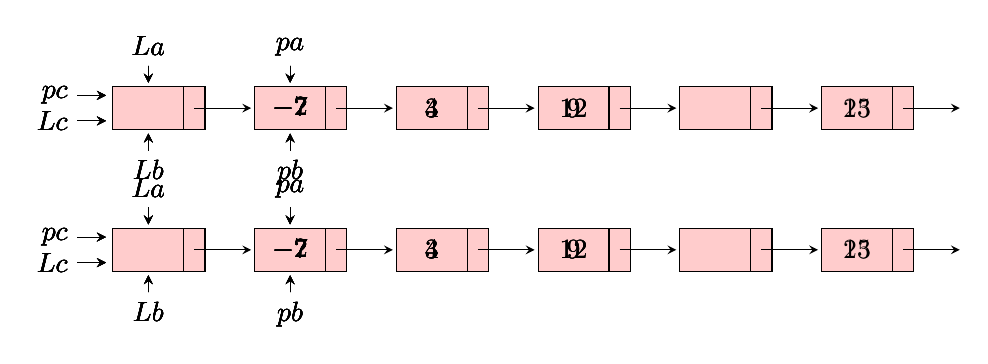
\begin{tikzpicture}[scale=0.9]
\def \x{1}
\def \y{0.6}

\foreach \c in {0,-2}{
\foreach \d in {0,2,4,6,8,10}{
\ifthenelse{  8 = \d }{
\node[left] at (\d+\x,\c+0.5*\y) {$\cd$};
}{
\filldraw[fill=red!20](\d+0,\c+0)rectangle(\d+\x,\c+\y);  
\filldraw[fill=red!20](\d+\x,\c+0)rectangle(\d+1.3*\x,\c+\y); 
}
\ifthenelse{  10 = \d}{

}{\draw[->,>=stealth] (\d+1.15*\x,\c+0.5*\y)--(\d+1.95*\x,\c+0.5*\y);}

\ifthenelse{ 0 = \c }{
\node[]at( 2.5,\c+0.5*\y){$-7$};
\node[]at( 4.5,\c+0.5*\y){$3$}; 
\node[]at( 6.5,\c+0.5*\y){$12$};
\node[]at(10.5,\c+0.5*\y){$23$};
\draw[->,>=stealth] (-.5*\x,\c+0.2*\y) node [left] {$Lc$}--(-0.1*\x,\c+0.2*\y);
\draw[->,>=stealth] (-.5,\c+0.8*\y) node[left] {$pc$}--(-.1*\x,\c+0.8*\y);
\draw[->,>=stealth] (2.5,\c+1.5*\y) node[above] {$pa$}--(2.5,\c+1.1*\y);
\draw[->,>=stealth] (0.5,\c+1.5*\y)node[above] {$La$} --(0.5,\c+1.1*\y);
}{
\node[]at( 2.5,\c+0.5*\y){$-2$};
\node[]at( 4.5,\c+0.5*\y){$4$}; 
\node[]at( 6.5,\c+0.5*\y){$9$};
\node[]at(10.5,\c+0.5*\y){$15$};
\draw[->,>=stealth] (2.5,\c-0.5*\y) node[below] {$pb$}--(2.5,\c-0.1*\y);
\draw[->,>=stealth] (0.5,\c-0.5*\y) node[below] {$Lb$}--(0.5,\c-0.1*\y);
}
}
}
\end{tikzpicture}
\caption{合并前的示意图}
\end{figure}